\subsection{What is Cisco ACI?}
ACI stands for Application Centric Infrastructure. It is a software-defined networking solution developed by Cisco Systems. It is designed to provide a centralized, policy-driven automation solution for managing and deploying applications across data center networks. ACI is built on a foundation of \textbf{software-defined networking (SDN)} principles, which separate the network control plane from the data plane, allowing for greater flexibility and agility in network management, in contrast to traditional networking solutions that are based on hardware-centric architectures.

Automation is achieved through the most crucial ACI feauture, the \textbf{Cisco APIC}. APIC also allows network scalability and flexibility, policy-based configuration and real-time monitoring and analytics. Compared to its traditional counterpart, APIC can be seen as a black box in the physical aspect of a network architecture. Any expansions or modifications to a network can be done by applying changes in the code. As a result, we will not have to worry about changing any hardware configurations or faulty equipment.

\begin{center}
    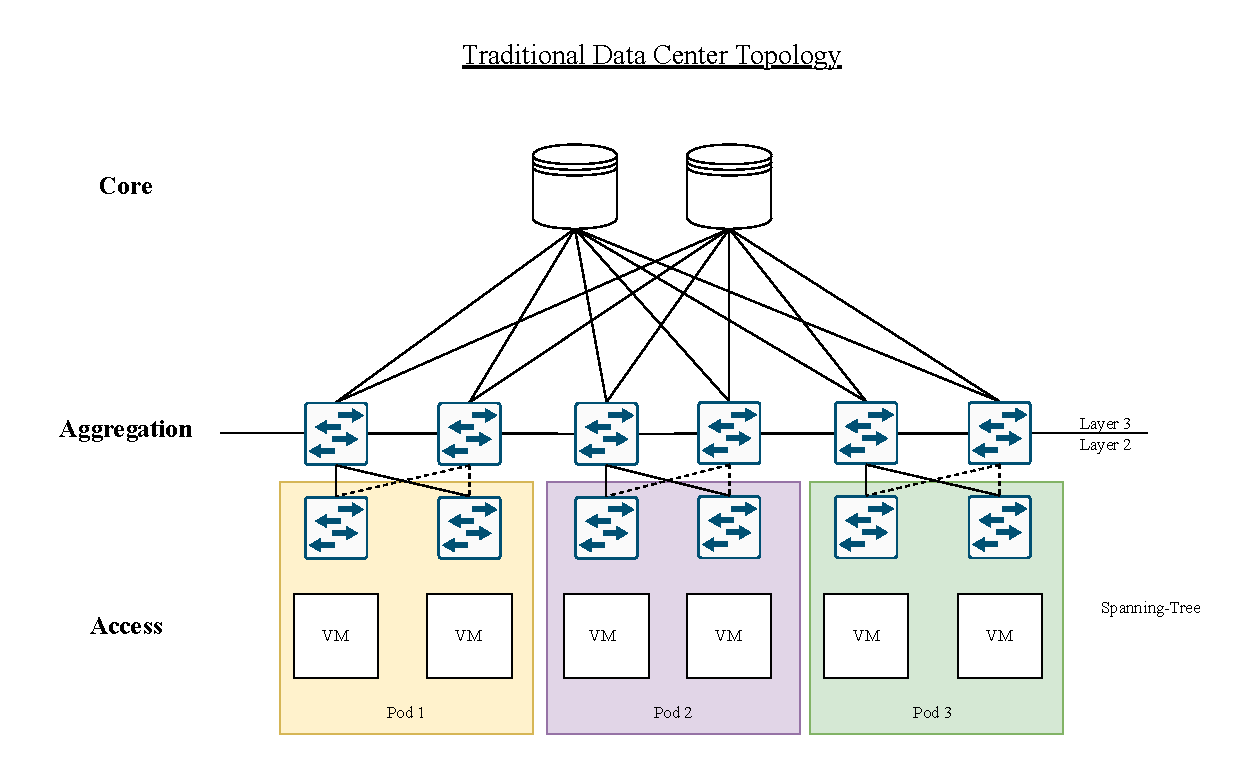
\includegraphics[scale=0.6]{Pics/traditional_topology.pdf}
\end{center}

\begin{note}
    \begin{center}
        \textbf{Spanning Tree Protocol}
        \textit{
            \\I think that I shall never see. A graph more lovely than a tree.\\
        A tree whose crucial property\\
        Is loop-free connectivity.\\
        A tree that must be sure to span.\\
        So packets can reach every LAN.\\
        First, the root must be selected.\\
        By ID, it is elected.\\
        Least cost paths from root are traced.\\
        In the tree, these paths are placed.\\
        A mesh is made by folks like me,\\
        Then bridges find a spanning tree.\\
        — Radia Perlman
        }
    \end{center}
    The goal of the Spanning Tree Protocol (STP) is to prevent loops in a network topology. This comes at the cost of bandwidth, as some links are blocked to prevent loops.
    \end{note}

Why is the traditional network architecture no longer sufficient for modern data centers? The traditional network architecture is based on a \textbf{three-tiered design, with core, distribution, and access layers}. This architecture is complex, rigid, and difficult to manage, especially in large-scale data center environments. It is also not well-suited for the dynamic nature of modern applications, which require rapid deployment and scaling of resources. In addition, traditional network architectures are not designed to support the growing trend of virtualization and cloud computing, which require a more flexible and scalable network infrastructure. Hardware devices such as routers, switches, and firewalls are manually configured and managed, which can be time-consuming and error-prone. In addition, traditional network architectures are not well-suited for the increasing demands of modern applications, which require high performance, low latency, and high availability. \textbf{ACI adds a layer of abstraction} to the network infrastructure, allowing for centralized management and automation of network policies. This enables organizations to deploy applications more quickly and efficiently, while also reducing the risk of human error and improving overall network performance and reliability.

\begin{center}
    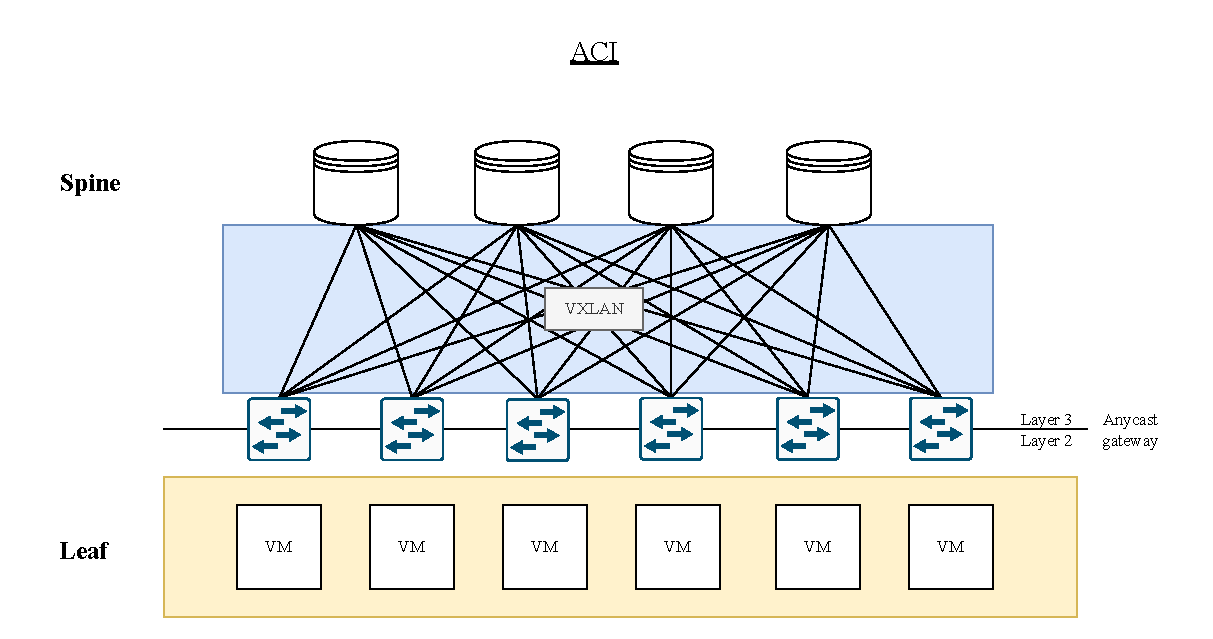
\includegraphics[scale=0.6]{Pics/aci_topology.pdf}
\end{center}

Cisco developed a 2-tier spine and leaf architecture, along with the VXLAN-based overlay system, which allowed for efficient handling of traffic between any two endpoints in the fabric and consistent latency for workloads.
\newpage
\begin{note}
    \begin{center}
        \textbf{VXLAN}
    \end{center}
    VXLAN allows you to create highly scalable logical networks with the support of multi-tenant broadcast domains and span physical network boundaries. These logical networks are overlay networks. When you decouple the virtual network from a physical network, you simplify the management of large networks, despite the complex initial configuration. When VXLAN is used, you can re-design the overlay network without needing to reconfigure the underlay (physical) network. It is possible to use two or more underlay L3 networks to deploy a virtual overlay L2 network domain. The Leaf-Spine network topology is a good solution for the underlay network to configure VXLAN overlay networks in large datacenters. Since L3 networks are used as the underlying network, \textbf{STP is not required}. This allows for a more efficient use of network resources.

   \begin{center}
    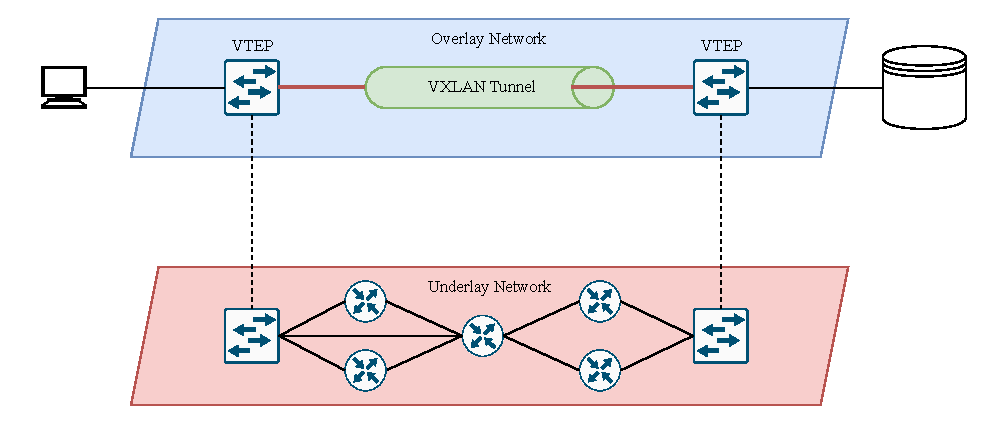
\includegraphics[scale=0.6]{Pics/vxlan.pdf}
   \end{center} 
\end{note}

Regarding security, ACI uses the \textbf{Zero Trust} security model. With the Zero Trust security model, even if the firewall allows some specific traffic in the network and regardless of where the request originates, it must still be verified. It works on the \textit{never trust, always verify} philosophy.

ACI provides the \textbf{Cisco Nexus Dashboard Platform}, an easy to scale, use and maintain platform that provides policy and connectivity automation, visibility, and analytics tools.